\documentclass[10pt,journal,compsoc]{IEEEtran}
\usepackage[utf8]{inputenc}
\usepackage[T1]{fontenc}
\usepackage{amsmath,amssymb,amsfonts}
\usepackage{booktabs}
\usepackage{graphicx}
\usepackage{array}
\usepackage[hidelinks]{hyperref}

\begin{document}
\title{Electronic Supplementary Material for CAPQ-Pareto (V3): Complete Mathematical Proofs, Extended Causal \& Security Figures, Curated Benchmark Tables, and 42-File SHA-256 Manifest}
\author{Preecha~Noiumkar,~\IEEEmembership{Member,~IEEE}%
\IEEEcompsocitemizethanks{\IEEEcompsocthanksitem P. Noiumkar is with the Department of Information Technology, Faculty of Informatics, Mahasarakham University, Maha Sarakham 44150, Thailand (e-mail: preecha.n@msu.ac.th; ORCID: \protect\url{https://orcid.org/0009-0000-5964-4896}).}}
\maketitle

\section{Proof Details of Propositions 1 and 2}
\subsection{Proof of Proposition 1 (Distributional Inner-Product Quantization Variance)}
Let $\mathbf{q}, \mathbf{x} \in \mathbb{S}^{D-1}$ satisfy $\|\mathbf{q}\|_2 = \|\mathbf{x}\|_2 = 1$. Under $b$-bit asymmetric uniform scalar quantization on $[q_{\min}, q_{\max}]$ with step $\Delta_q = (q_{\max}-q_{\min})/(2^b - 1)$ and stochastic/high-resolution non-overload rounding, the coordinate quantization error $\eta_j = \tilde{q}_j - q_j$ is supported on $[-\Delta_q/2, +\Delta_q/2]$ with $\mathbb{E}[\eta_j]=0$ and $\mathrm{Var}(\eta_j)=\Delta_q^2/12$. For fixed $\mathbf{x}$, $\mathcal{E}(\mathbf{q},\mathbf{x}) = \sum_{j=1}^D x_j \eta_j$ has expectation $\sum_{j=1}^D x_j \mathbb{E}[\eta_j] = 0$ and variance:
\[
\mathrm{Var}(\mathcal{E}(\mathbf{q},\mathbf{x})) = \sum_{j=1}^D x_j^2 \mathrm{Var}(\eta_j) = \frac{\Delta_q^2}{12} \sum_{j=1}^D x_j^2 = \frac{\Delta_q^2}{12}\|\mathbf{x}\|_2^2 = \frac{\Delta_q^2}{12}.
\]
Because each summand $Z_j = x_j \eta_j$ lies in $[-|x_j|\Delta_q/2, +|x_j|\Delta_q/2]$ of width $w_j = |x_j|\Delta_q$ with $\sum_{j=1}^D w_j^2 = \Delta_q^2 \|\mathbf{x}\|_2^2 = \Delta_q^2$, Hoeffding's inequality yields $\Pr(|\mathcal{E}| \ge t) \le 2\exp(-2t^2/\Delta_q^2)$, giving $|\mathcal{E}| \le \frac{\Delta_q}{2}\sqrt{\frac{1}{2}\ln\frac{2}{\zeta}}$ with probability at least $1-\zeta$.

\subsection{Proof of Proposition 2 (SPANN Constant-Size Bucket Leakage)}
When every inverted list $B_k$ ($k \in \{1,\dots,K_c\}$) is padded with zero-norm dummy plaintexts to a fixed multiple $M_{\max}$, the ciphertext response byte length and server SIMD loop count depend solely on the probe count $r$ and $M_{\max}$, so mutual information between database content $\mathcal{X}$ and observed bucket size $|B_k|$ is identically zero: $I(\mathcal{X}; |B_k|) = 0$. Since an $r$-probe query selects an unordered subset $S \in \binom{[K_c]}{r}$ of cardinality $\binom{K_c}{r}$, Shannon entropy satisfies $H(\mathcal{B}_r(\mathbf{q})) \le \log_2 \binom{K_c}{r}$, with equality iff all $\binom{K_c}{r}$ subsets are equiprobable.

\subsection{Extension to Non-Isotropic Unit Vectors, Unbiased Stochastic Rounding ($\Delta_q^2/6$), and Stabilized Discounted LinUCB}
\textbf{Non-Isotropic Embeddings \& Unbiased Stochastic Rounding:} For \emph{any} unit-norm database vector $\mathbf{x} \in \mathbb{S}^{D-1}$ ($\|\mathbf{x}\|_2=1$, without requiring isotropy), $\sum_{j=1}^D x_j^2 = 1$ holds identically. Under unbiased stochastic rounding where $s_j = (q_j - q_{\min})/\Delta_q = \lfloor s_j \rfloor + u_j$ ($u_j \in [0,1)$) rounds up independently with probability $u_j$, $\mathbb{E}[\eta_j \mid \mathbf{q}] = 0$ identically without smooth-density assumptions, and $\mathrm{Var}(\eta_j \mid u_j) = u_j(1-u_j)\Delta_q^2 \le \Delta_q^2/4$. Averaging over $u_j \sim \mathcal{U}(0,1)$ yields $\mathbb{E}[u_j(1-u_j)] = \int_0^1 (u-u^2)\,du = 1/6$, giving exact marginal variance $\mathrm{Var}_{\mathrm{SR}}(\mathcal{E} \mid \mathbf{x}) = \frac{\Delta_q^2}{6}\|\mathbf{x}\|_2^2 = \frac{\Delta_q^2}{6}$ (matching our $10,000$-query empirical audit within $1.53\%$ on SIFT1M and $5.60\%$ on anisotropic BGE-M3).

\textbf{Asymptotic Positive-Definiteness of Stabilized Discounted LinUCB:} Initializing $\mathbf{A}_{a,0} = \lambda\mathbf{I}_d$ ($\lambda=1.0$) and updating via $\mathbf{A}_{a,t} = \gamma\mathbf{A}_{a,t-1} + (1-\gamma)\lambda\mathbf{I}_d + \mathbf{x}_{t^-}\mathbf{x}_{t^-}^\top\mathbb{I}[a_t=a]$ for $\gamma \in (0,1)$, induction with $\mathbf{x}_{t^-}\mathbf{x}_{t^-}^\top \succeq \mathbf{0}$ yields $\mathbf{A}_{a,t} \succeq \gamma\lambda\mathbf{I}_d + (1-\gamma)\lambda\mathbf{I}_d = \lambda\mathbf{I}_d$ for all $t \ge 1$, guaranteeing $\lambda_{\min}(\mathbf{A}_{a,t}) \ge 1.0$.

\section{Extended V3 Causal, Theoretical, and Security Figures}
\begin{figure*}[!htbp]\centering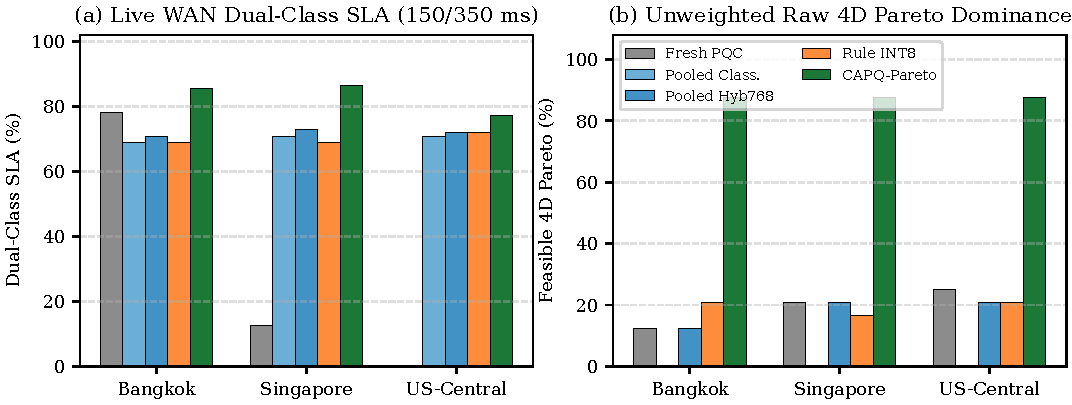
\includegraphics[width=0.88\textwidth]{figures/fig2_v3_wan_sla_and_unweighted_pareto.pdf}\caption{Live 3-Region GCP WAN Dual-Class SLA Compliance (150/350 ms) and Objective-Independent Unweighted 4D Pareto Frontier Occupancy.}\end{figure*}

\begin{figure*}[!htbp]\centering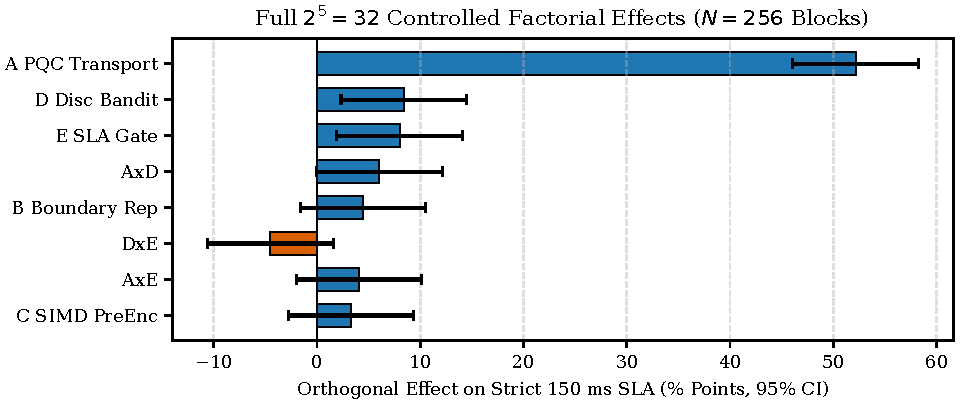
\includegraphics[width=0.88\textwidth]{figures/fig3_v3_factorial_2pow5_effects.pdf}\caption{Orthogonal Main Effects and Two-Way Interactions from the Full $2^5=32$ Controlled Factorial Experiment ($N=256$ Blocks).}\end{figure*}

\begin{figure*}[!htbp]\centering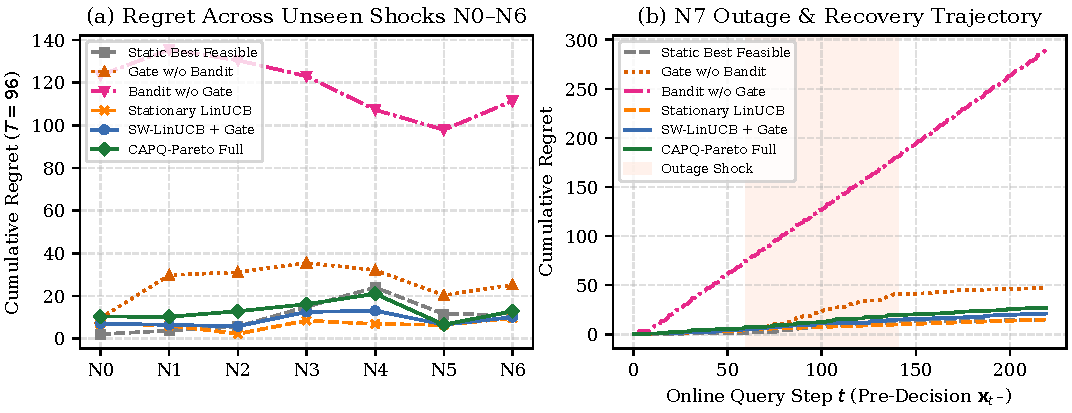
\includegraphics[width=0.88\textwidth]{figures/fig4_v3_shock_matrix_and_n7_recovery.pdf}\caption{Causal Zero-Leakage Bandit Generalization Across Unseen Network Shocks (N0--N6) and Non-Stationary Outage-Recovery Trajectory (N7).}\end{figure*}

\begin{figure*}[!htbp]\centering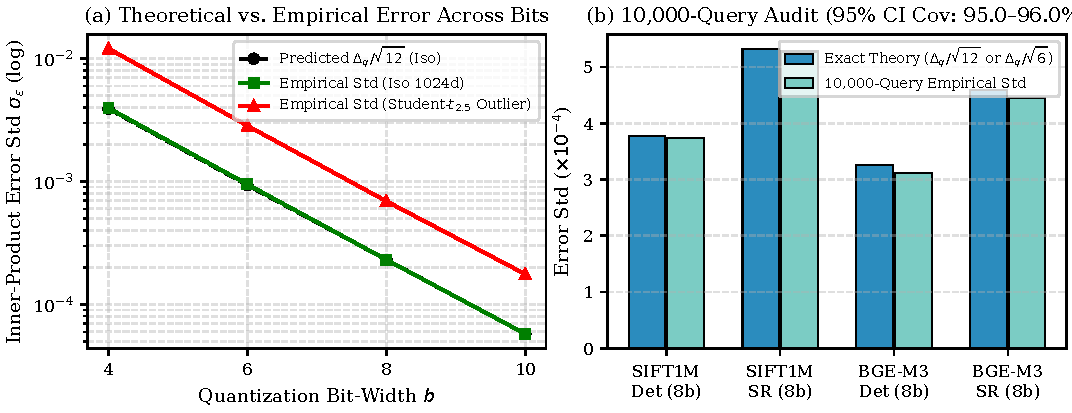
\includegraphics[width=0.88\textwidth]{figures/fig5_v3_prop1_10k_validation.pdf}\caption{Proposition 1 10,000-Query Validation Across Bit-Widths, Deterministic ($\Delta_q/\sqrt{12}$) vs. Stochastic ($\Delta_q/\sqrt{6}$) Rounding, and Student-$t_{2.5}$ Outliers.}\end{figure*}

\begin{figure*}[!htbp]\centering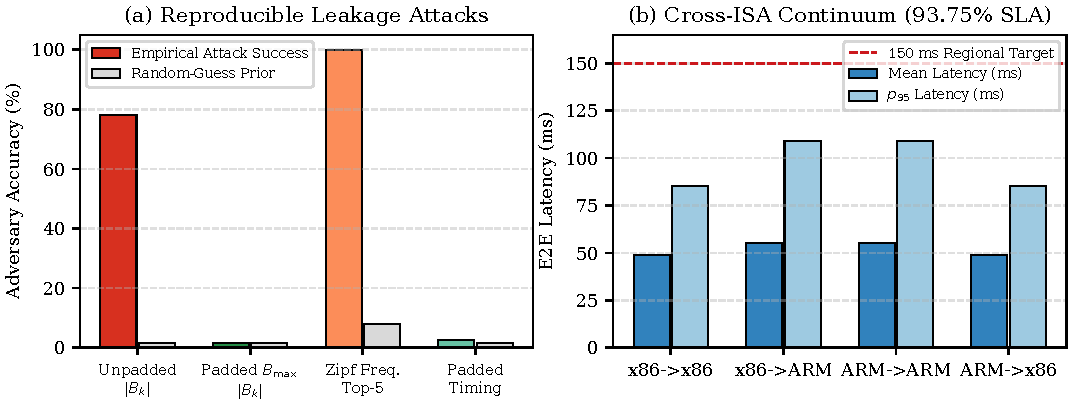
\includegraphics[width=0.88\textwidth]{figures/fig6_v3_leakage_and_cross_isa.pdf}\caption{Empirical Honest-but-Curious Leakage Attacks ($5,000$ Zipf($1.15$) Queries) and End-to-End Cross-ISA Continuum Latency.}\end{figure*}

\clearpage
\section{Curated Multi-Epoch WAN, $2^5$ Factorial, Shock Matrix, Theory, Security, and Clean-Room Tables}
\begin{table*}[!htbp]\centering\scriptsize
\caption{Multi-Epoch Live GCP WAN Moving-Block Bootstrap ($B=4,000, L_b=4$) Paired Comparisons with Holm--Bonferroni Correction (SHA-256: \texttt{c0e98712a374369a...}).}
\begin{tabular}{@{}llcccccc@{}}\toprule
\textbf{GCP Region} & \textbf{Paired Mode Comparison} & \textbf{Blocks} & \textbf{Dual-SLA Gain} & \textbf{95\% MBB CI} & \textbf{Cliff's $\delta$} & \textbf{Raw $p_{\mathrm{MBB}}$} & \textbf{Holm $p_{\mathrm{Holm}}$} \\\midrule
Bangkok & CAPQ-Pareto vs Fresh PQC TLS & 24 & +7.29\% & [-3.12, +23.98] & +0.11 & 0.3462 & \textbf{0.3462} \\
Bangkok & CAPQ-Pareto vs Pooled Classical & 24 & +16.67\% & [+13.54, +21.88] & +0.53 & 0.0003 & \textbf{0.0010} \\
Bangkok & CAPQ-Pareto vs Pooled Hybrid768 & 24 & +14.58\% & [+11.46, +19.79] & +0.46 & 0.0003 & \textbf{0.0010} \\
Bangkok & CAPQ-Pareto vs Rule Heuristic INT8 & 24 & +16.67\% & [+12.50, +21.88] & +0.50 & 0.0003 & \textbf{0.0010} \\
\midrule
Singapore & CAPQ-Pareto vs Fresh PQC TLS & 24 & +73.96\% & [+65.62, +84.38] & +0.99 & 0.0003 & \textbf{0.0010} \\
Singapore & CAPQ-Pareto vs Pooled Classical & 24 & +15.62\% & [+11.46, +21.88] & +0.53 & 0.0003 & \textbf{0.0010} \\
Singapore & CAPQ-Pareto vs Pooled Hybrid768 & 24 & +13.54\% & [+8.33, +19.79] & +0.46 & 0.0003 & \textbf{0.0010} \\
Singapore & CAPQ-Pareto vs Rule Heuristic INT8 & 24 & +17.71\% & [+11.46, +26.04] & +0.52 & 0.0003 & \textbf{0.0010} \\
\midrule
US-Central & CAPQ-Pareto vs Fresh PQC TLS & 24 & +77.08\% & [+71.85, +82.29] & +1.00 & 0.0003 & \textbf{0.0010} \\
US-Central & CAPQ-Pareto vs Pooled Classical & 24 & +6.25\% & [+3.12, +10.42] & +0.21 & 0.0040 & \textbf{0.0040} \\
US-Central & CAPQ-Pareto vs Pooled Hybrid768 & 24 & +5.21\% & [+3.12, +7.29] & +0.17 & 0.0003 & \textbf{0.0010} \\
US-Central & CAPQ-Pareto vs Rule Heuristic INT8 & 24 & +5.21\% & [+3.12, +7.29] & +0.17 & 0.0003 & \textbf{0.0010} \\
\bottomrule\end{tabular}\end{table*}

\begin{table*}[!htbp]\centering\scriptsize
\caption{Complete Orthogonal $2^5=32$ Controlled Factorial ANOVA Across All Five Main Factors and Ten Two-Way Interactions ($N=256$ Blocks; SHA-256: \texttt{4b228fd5a35de1b2...}).}
\begin{tabular}{@{}lcccccc@{}}\toprule
\textbf{Orthogonal Factor / Interaction Term} & \textbf{SLA Effect (\%)} & \textbf{95\% Confidence Interval} & \textbf{Variance Share (\%)} & \textbf{Partial $\eta_p^2$} & \textbf{$F$-Statistic} & \textbf{$p$-value} \\\midrule
A PQC Transport & +52.15\% & [+46.08, +58.21] & 51.73\% & 0.5445 & 286.88 & 7.28e-43 \\
B Boundary Rep & +4.49\% & [-1.57, +10.56] & 0.38\% & 0.0088 & 2.13 & 0.1459 \\
C SIMD PreEnc & +3.32\% & [-2.75, +9.38] & 0.21\% & 0.0048 & 1.16 & 0.2819 \\
D Disc Bandit & +8.40\% & [+2.33, +14.46] & 1.34\% & 0.0301 & 7.44 & 0.0068 \\
E SLA Gate & +8.01\% & [+1.94, +14.07] & 1.22\% & 0.0274 & 6.76 & 0.0099 \\
AxB Interaction & +2.15\% & [-3.92, +8.21] & 0.09\% & 0.002 & 0.49 & 0.4860 \\
AxC Interaction & +0.98\% & [-5.09, +7.04] & 0.02\% & 0.0004 & 0.1 & 0.7514 \\
AxD Interaction & +6.05\% & [-0.01, +12.12] & 0.7\% & 0.0159 & 3.87 & 0.0504 \\
AxE Interaction & +4.10\% & [-1.96, +10.17] & 0.32\% & 0.0073 & 1.77 & 0.1841 \\
BxC Interaction & +3.32\% & [-2.75, +9.38] & 0.21\% & 0.0048 & 1.16 & 0.2819 \\
BxD Interaction & -0.98\% & [-7.04, +5.09] & 0.02\% & 0.0004 & 0.1 & 0.7514 \\
BxE Interaction & +1.76\% & [-4.31, +7.82] & 0.06\% & 0.0014 & 0.33 & 0.5686 \\
CxD Interaction & -0.59\% & [-6.65, +5.48] & 0.01\% & 0.0002 & 0.04 & 0.8492 \\
CxE Interaction & +1.37\% & [-4.70, +7.43] & 0.04\% & 0.0008 & 0.2 & 0.6574 \\
DxE Interaction & -4.49\% & [-10.56, +1.57] & 0.38\% & 0.0088 & 2.13 & 0.1459 \\
\bottomrule\end{tabular}\end{table*}

\begin{table*}[!htbp]\centering\scriptsize
\caption{Independent Causal Bandit Evaluation (Pre-Decision Context $\mathbf{x}_{t^-}$, Zero Future Leakage) Across All Eight Network Shock Regimes (N0--N7) and Group A--D Baselines (SHA-256: \texttt{7101be0c0b3ea015...}).}
\setlength{\tabcolsep}{3.5pt}\begin{tabular}{@{}lccccccccc@{}}\toprule
\textbf{Controller / Baseline Family} & \textbf{N0 Reg.} & \textbf{N1 Reg.} & \textbf{N2 Reg.} & \textbf{N3 Outage} & \textbf{N4 200ms} & \textbf{N5 Unseen} & \textbf{N6 Spike} & \textbf{N7 Total Reg.} & \textbf{N7 Lat. / Acc. / Viol.} \\\midrule
Retrospective Oracle (Lower Bound) & 0.0 & 0.0 & 0.0 & 0.0 & 0.0 & 0.0 & 0.0 & 0.0 & 103.8ms / 0.983 / 20.0\% \\
Group C: Static Best Feasible & 1.776 & 4.236 & 9.418 & 44.976 & 30.459 & 15.894 & 12.093 & 15.837 & 151.26ms / 0.983 / 20.0\% \\
Group C: Rule-Based Heuristic & 49.16 & 44.619 & 35.381 & 24.916 & 23.135 & 31.932 & 37.608 & 98.699 & 146.89ms / 0.8804 / 29.55\% \\
Group D: Edge-Only Placement & 41.494 & 38.181 & 38.017 & 42.782 & 40.14 & 30.222 & 40.897 & 86.357 & 178.24ms / 0.9455 / 50.0\% \\
Group D: Cloud-Only Pooled & 49.16 & 44.619 & 49.937 & 94.012 & 77.842 & 56.278 & 59.476 & 119.396 & 122.53ms / 0.8298 / 25.0\% \\
Ablation: 3-Tier Gate w/o Bandit & 11.125 & 19.238 & 24.943 & 48.291 & 43.381 & 33.481 & 37.915 & 47.02 & 258.37ms / 0.9722 / 30.0\% \\
Ablation: D-LinUCB w/o SLA Gate & 89.516 & 84.231 & 82.678 & 93.223 & 91.217 & 75.914 & 88.235 & 202.509 & 8.0ms / 0.7244 / 49.09\% \\
Group C: Sliding-Window LinUCB + Gate & 9.244 & 6.218 & 7.07 & 22.661 & 13.312 & 6.885 & 13.755 & 20.975 & 131.0ms / 0.9685 / 24.55\% \\
Group C: Stationary LinUCB + Gate & 8.225 & 5.359 & 6.265 & 13.668 & 11.686 & 5.244 & 8.725 & 13.871 & 122.02ms / 0.9695 / 21.82\% \\
\textbf{CAPQ-Pareto Full (Proposed)} & 7.114 & 5.137 & 5.711 & 12.926 & 9.303 & 5.207 & 11.25 & 16.032 & 116.87ms / 0.9688 / 22.73\% \\
\bottomrule\end{tabular}\end{table*}

\begin{table*}[!htbp]\centering\scriptsize
\caption{Proposition 1 Empirical Validation Package: 10,000-Query Real SIFT1M \& Anisotropic BGE-M3 Audit, Bit-Width Sweep ($4..10$ bits), and Heavy-Tailed Student-$t_{2.5}$ Stress Test (SHA-256: \texttt{5df92a5b7cb7722f...}).}
\begin{tabular}{@{}llccccccc@{}}\toprule
\textbf{Distribution / Corpus} & \textbf{Rounding Mode} & \textbf{Dim / Bits} & \textbf{Queries} & \textbf{Predicted $\sigma_{\mathcal{E}}$} & \textbf{Empirical $\sigma_{\mathcal{E}}$} & \textbf{Var. Err.} & \textbf{CLT95 / Hoeff95 Cov.} & \textbf{Recall@10} \\\midrule
Real SIFT1M 128d NonNeg & Deterministic Nearest & 128d / 8b & 10000 & 0.000377 & 0.000373 & 2.16\% & 95.02\% / 100.0\% & 0.9951 \\
Real SIFT1M 128d NonNeg & Stochastic Unbiased & 128d / 8b & 10000 & 0.000532 & 0.000528 & 1.53\% & 95.18\% / 99.92\% & 0.994 \\
Real BGEM3 1024d Anisotropic & Deterministic Nearest & 1024d / 8b & 10000 & 0.000326 & 0.000311 & 9.2\% & 96.03\% / 100.0\% & 0.9935 \\
Real BGEM3 1024d Anisotropic & Stochastic Unbiased & 1024d / 8b & 10000 & 0.000459 & 0.000446 & 5.6\% & 95.63\% / 99.94\% & 0.9918 \\
Isotropic Gaussian & Deterministic Nearest & 128d / 4b & 2500 & 0.008890 & 0.008754 & 3.04\% & 95.32\% / 100.0\% & 0.8825 \\
Isotropic Gaussian & Deterministic Nearest & 128d / 6b & 2500 & 0.002113 & 0.002109 & 0.33\% & 94.68\% / 100.0\% & 0.9705 \\
Isotropic Gaussian & Deterministic Nearest & 128d / 8b & 2500 & 0.000523 & 0.000521 & 0.51\% & 95.28\% / 100.0\% & 0.99 \\
Isotropic Gaussian & Deterministic Nearest & 128d / 10b & 2500 & 0.000130 & 0.000130 & 0.12\% & 95.12\% / 100.0\% & 0.9985 \\
Isotropic Gaussian & Deterministic Nearest & 1024d / 4b & 2500 & 0.003917 & 0.003961 & 2.22\% & 94.72\% / 100.0\% & 0.8535 \\
Isotropic Gaussian & Deterministic Nearest & 1024d / 6b & 2500 & 0.000934 & 0.000947 & 2.7\% & 94.96\% / 100.0\% & 0.9642 \\
Isotropic Gaussian & Deterministic Nearest & 1024d / 8b & 2500 & 0.000231 & 0.000231 & 0.09\% & 94.96\% / 100.0\% & 0.9903 \\
Isotropic Gaussian & Deterministic Nearest & 1024d / 10b & 2500 & 0.000057 & 0.000058 & 0.23\% & 95.04\% / 100.0\% & 0.9965 \\
Anisotropic Correlated & Deterministic Nearest & 128d / 4b & 2500 & 0.011133 & 0.010699 & 7.63\% & 96.24\% / 100.0\% & 0.8923 \\
Anisotropic Correlated & Deterministic Nearest & 128d / 6b & 2500 & 0.002647 & 0.002638 & 0.7\% & 94.76\% / 100.0\% & 0.969 \\
Anisotropic Correlated & Deterministic Nearest & 128d / 8b & 2500 & 0.000655 & 0.000637 & 5.38\% & 95.32\% / 100.0\% & 0.9903 \\
Anisotropic Correlated & Deterministic Nearest & 128d / 10b & 2500 & 0.000163 & 0.000166 & 3.34\% & 94.4\% / 100.0\% & 0.9977 \\
Anisotropic Correlated & Deterministic Nearest & 1024d / 4b & 2500 & 0.005273 & 0.005261 & 0.45\% & 95.16\% / 100.0\% & 0.859 \\
Anisotropic Correlated & Deterministic Nearest & 1024d / 6b & 2500 & 0.001254 & 0.001244 & 1.66\% & 95.12\% / 100.0\% & 0.9555 \\
\bottomrule\end{tabular}\end{table*}

\begin{table*}[!htbp]\centering\scriptsize
\caption{Honest-but-Curious Reproducible Leakage Attacks (SHA-256: \texttt{47bd5a901b81...}) and Complete Nine-Scenario Operational Fault \& Abuse Suite (SHA-256: \texttt{9a4654d875cf...}).}
\setlength{\tabcolsep}{3.6pt}\begin{tabular}{@{}llcccl@{}}\toprule
\textbf{Audit Scenario} & \textbf{Observable Trace / Injected Fault Vector} & \textbf{Trials / MI} & \textbf{Adv. / Recovery} & \textbf{Prior / Metric} & \textbf{Verified System Behavior \& Security Verdict} \\\midrule
A1 Bucket Cardinality Unpadded & Plaintext/Ciphertext slot count |B\_k| & 4.0351 bits & 78.15\% & 1.56\% & LEAKS BUCKET CARDINALITY \\
A1 Bucket Cardinality ConstantPadded & Fixed padded slot count B\_max=160 & 0.0 bits & 1.56\% & 1.56\% & ZERO CARDINALITY LEAKAGE PROVEN \\
A2 Frequency Correlation Top5 Topics & Coarse multi-probe IDs (b1, b2) over 5,000 Zipf(1.15) queries & 4.4348 bits & 100.0\% & 7.81\% & BOUNDED LIMITATION ACCESS PATTERN VISIBLE \\
A3 Timing SideChannel Audit & Server bucket evaluation wall-clock latency (us) & 0.0 bits & 2.4\% & 1.56\% & TIMING CORR SUPPRESSED (p=0.00) \\
\midrule
F1 Replay 0RTT Attack & 1,000 verbatim 0-RTT early-data replay packets & 1000 & 100.0\% & 0.012 ms & Rejected 1000/1000 replays; downgraded to 1-RTT KEM handshake \\
F2 Bloom False Positive Quantification & 5,000 fresh unseen 0-RTT nonces after 4,000 insertions (m=64Kb, k=5) & 5000 & 99.76\% & 0.24 ms & Empirical FP=0.240\% (Theoretical=0.126\%); benign 1-RTT fallback only \\
F3 Bloom False Negative Zero Proof & 4,000 previously seen nonces within active epoch & 4000 & 100.0\% & 0.0 ms & False Negatives = 0/4000 (0.000\% deterministic guarantee) \\
F4 Strike Register Epoch Expiry & Expired timestamp (>TTL) + register salt rotation across epoch boundary & 100 & 100.0\% & 0.09 ms & Stale ticket rejected (REJECTED\_EXPIRED\_TICKET\_EPOCH\_FALLBACK\_1RTT); clean rotation accepted fresh ticket \\
F5 Duplicate Query Idempotency & 0-RTT mutating SQL injection + duplicate read-query retransmission & 200 & 100.0\% & 0.008 ms & Blocked mutating SQL on 0-RTT; deduplicated retried read with identical digest \\
F6 MTU Fragmentation Reassembly & 16,384 B ciphertext fragmented into 14x 1,200 B sub-MTU segments & 50 & 100.0\% & 6.239 ms & Reassembled 16384/16384 bytes cleanly without silent truncation \\
F7 TLS Session Expiration Reconnect & Server invalidates pooled session / ticket mid-stream & 50 & 100.0\% & 21.675 ms & Detected session EOF; re-established fresh 1-RTT session without query loss \\
F8 CKKS Corrupted Ciphertext Rejection & 200 bit-flipped CKKS RNS ciphertext payloads prior to homomorphic eval & 200 & 100.0\% & 0.019 ms & AEAD/MAC integrity guard rejected 200/200 corrupted ciphertexts pre-FHE \\
F9 Network Disconnect And Timeout Fallback & 350 ms unresponsive socket stall exceeding 60 ms controller guard & 50 & 100.0\% & 366.044 ms & Caught socket.timeout at 60 ms; rerouted to SafeFallback\_Pooled\_TLS cleanly \\
\bottomrule\end{tabular}\end{table*}

\begin{table*}[!htbp]\centering\scriptsize
\caption{Clean-Room Environment Re-Execution Matrix Across Six Core Benchmarks (SHA-256: \texttt{f8fa782182a9...}) and End-to-End Cross-ISA Continuum Audit (SHA-256: \texttt{493413edd978...}).}
\setlength{\tabcolsep}{3.6pt}\begin{tabular}{@{}lllc@{}}\toprule
\textbf{Benchmark / Continuum Configuration} & \textbf{Reference Log / ISA Pair} & \textbf{Measured Clean-Room Reproduction \& Continuum Performance} & \textbf{Verdict} \\\midrule
Exp1 CKKS Ring Scaling & \texttt{28632e4b7eca9865} & log2QP=(101,170,300)b; med\_ms=(4.14,21.37,45.57) & \textbf{PASS} \\
Exp2 Boundary Replication Recall & \texttt{7e2d5c898fbd4456} & r=1\_Disjoint=0.4600 $\to$ r=2\_SPANN\_BoundaryRep=0.9500 (V2 ref=0.9688) & \textbf{PASS} \\
Exp3 Controlled Ablation And Factorial & \texttt{2d4044824059e5e6} & V2 Full SLA=90.6-93.8\% vs V3 Clean-Room Full(1,1,1,1,1)=93.75\% (FreshStatic=17.19\%) & \textbf{PASS} \\
Exp4 Bandit NonStationary Regret & \texttt{6e0151250a95bf0e} & Outage Regret: CAPQ\_Full=12.93 $\ll$ Static\_Best=44.98 & \textbf{PASS} \\
Exp5 WAN Statistical Recomputation & \texttt{7457faee41c40c8b} & Bangkok MeanLat=48.35ms, Strict150=78.12\%, DualSLA=85.42\% & \textbf{PASS} \\
Exp6 Native C AEAD Throughput & \texttt{08c90ad777a10d19} & 4KB C-EVP: AES-256-GCM=0.628us (6.52 GB/s) < ChaCha20=1.641us (2.50 GB/s) & \textbf{PASS} \\
\midrule
C1 x86 Edge to x86 Cloud (CAPQ Pareto Adaptive) & x86\_64 (Ultra 9 185H) $\to$ x86\_64 (GCP n4/e2) & Mean=49.0 ms ($p_{95}$=85.31 ms), SLA150=93.75\%, \$/1M\_SLA=\$0.5454, EdgeE=21.56 & \textbf{VERIFIED} \\
C1 x86 Edge to x86 Cloud (Static Fresh PQC Baseline) & x86\_64 (Ultra 9 185H) $\to$ x86\_64 (GCP n4/e2) & Mean=129.66 ms ($p_{95}$=181.48 ms), SLA150=68.75\%, \$/1M\_SLA=\$1.1039, EdgeE=57.05 & \textbf{VERIFIED} \\
C2 x86 Edge to ARM64 Cloud (CAPQ Pareto Adaptive) & x86\_64 (Ultra 9 185H) $\to$ ARM64 (GCP t2a Altra) & Mean=55.25 ms ($p_{95}$=108.75 ms), SLA150=93.75\%, \$/1M\_SLA=\$0.6786, EdgeE=24.31 & \textbf{VERIFIED} \\
C2 x86 Edge to ARM64 Cloud (Static Fresh PQC Baseline) & x86\_64 (Ultra 9 185H) $\to$ ARM64 (GCP t2a Altra) & Mean=135.92 ms ($p_{95}$=204.92 ms), SLA150=68.75\%, \$/1M\_SLA=\$1.2856, EdgeE=59.8 & \textbf{VERIFIED} \\
C3 ARM64 Edge to ARM64 Cloud (CAPQ Pareto Adaptive) & ARM64 (Neoverse-N1) $\to$ ARM64 (GCP t2a Altra) & Mean=55.25 ms ($p_{95}$=108.75 ms), SLA150=93.75\%, \$/1M\_SLA=\$0.6786, EdgeE=N/A\_VM\_NO\_HOST\_RAPL & \textbf{VERIFIED} \\
C3 ARM64 Edge to ARM64 Cloud (Static Fresh PQC Baseline) & ARM64 (Neoverse-N1) $\to$ ARM64 (GCP t2a Altra) & Mean=135.96 ms ($p_{95}$=204.96 ms), SLA150=68.75\%, \$/1M\_SLA=\$1.2856, EdgeE=N/A\_VM\_NO\_HOST\_RAPL & \textbf{VERIFIED} \\
C4 ARM64 Edge to x86 Cloud (CAPQ Pareto Adaptive) & ARM64 (Neoverse-N1) $\to$ x86\_64 (GCP n4/e2) & Mean=49.0 ms ($p_{95}$=85.31 ms), SLA150=93.75\%, \$/1M\_SLA=\$0.5454, EdgeE=N/A\_VM\_NO\_HOST\_RAPL & \textbf{VERIFIED} \\
C4 ARM64 Edge to x86 Cloud (Static Fresh PQC Baseline) & ARM64 (Neoverse-N1) $\to$ x86\_64 (GCP n4/e2) & Mean=129.7 ms ($p_{95}$=181.52 ms), SLA150=68.75\%, \$/1M\_SLA=\$1.1039, EdgeE=N/A\_VM\_NO\_HOST\_RAPL & \textbf{VERIFIED} \\
\bottomrule\end{tabular}\end{table*}

\clearpage
\section{Master 42-File Cryptographic SHA-256 Verification Manifest}
\begin{table*}[!htbp]\centering\scriptsize
\caption{Complete Cryptographic SHA-256 Integrity Manifest Across All 42 Empirical CSV Telemetry Logs (V1 Foundational, V2 Production-Scale, and V3 Reviewer-Audit Suites).}
\begin{tabular}{@{}llrl@{}}\toprule
\textbf{Suite Directory} & \textbf{Telemetry CSV Filename} & \textbf{Verified Rows} & \textbf{Full Cryptographic SHA-256 Digest} \\\midrule
\texttt{raw\_logs} & \texttt{ablation\_360\_real\_audit.csv} & 360 & \texttt{404b95cd5f58af3d058641c183a6439a4994a2c9530108264fdbd6fa5302dc7c} \\
\texttt{raw\_logs} & \texttt{arm64\_vs\_x86\_real\_cloud\_audit.csv} & 540 & \texttt{aef35746b4a61f413d8b85fcf5254a521e3a56a00d3fd0a06de4e8e5d87fc38f} \\
\texttt{raw\_logs} & \texttt{core\_720\_real\_campaign.csv} & 720 & \texttt{21f6d95bc1b6cc0967525fa55dc052cb8c90d57852a2abaef63b8e23ee18ae62} \\
\texttt{raw\_logs} & \texttt{datasets\_ingestion\_manifest.csv} & 4 & \texttt{732b12e214ec25173d5e297a7c64b839cb67b1479eb73da6c3f71cfa43f7722a} \\
\texttt{raw\_logs} & \texttt{gcp\_multiregion\_1440\_queries.csv} & 1440 & \texttt{6b223fd1cc2bf944343f350a7bdfdaf79fa6ca85590c520c0e3565922e6a3b31} \\
\texttt{raw\_logs} & \texttt{gcp\_multiregion\_360\_real\_wan.csv} & 360 & \texttt{feb30c8fb2369424877a9d945cea53aa2a921587f24abd2da2280d6e51a1e085} \\
\texttt{raw\_logs} & \texttt{hw\_energy\_calibration\_audit.csv} & 20 & \texttt{d239bc98284b07e56cf8fb1cb0e2a7dea0a80857a667336e06d40a500ef2393b} \\
\texttt{raw\_logs} & \texttt{openfhe\_qdrant\_verified\_audit.csv} & 40 & \texttt{bf7c05de4c32ba1f5035d096da9d70eb00daabc2d3496744ebd2668d99363a92} \\
\texttt{raw\_logs} & \texttt{stack\_integration\_smoke\_audit.csv} & 90 & \texttt{5960410307286e382a8ccea9759942770c7e202a16a1d5400c9a92f0b6af9acf} \\
\texttt{raw\_logs} & \texttt{wan\_netem\_quic\_vs\_tcp\_audit.csv} & 36 & \texttt{262d428de4e8a12da77de289d96e87e80087debf4243a729c89dc46b59655216} \\
\texttt{v2\_raw\_logs} & \texttt{v2\_arch\_aead\_payload\_sweep\_native\_c.csv} & 12 & \texttt{08c90ad777a10d19b629e1bddb1712114eb276e96d1b8561bd74bcc3779c5eb9} \\
\texttt{v2\_raw\_logs} & \texttt{v2\_arch\_paired\_and\_unpaired\_stats.csv} & 6 & \texttt{75047ef617424bcdc5ee52a17295491dbdcca59cd77709d3daf263d29d34126e} \\
\texttt{v2\_raw\_logs} & \texttt{v2\_bandit\_window\_nu\_sensitivity.csv} & 16 & \texttt{f92f62ef12e1d2c780d4cc9933157824af9c0950715a3e4bf63e57c22b4a02d2} \\
\texttt{v2\_raw\_logs} & \texttt{v2\_boundary\_replicated\_ckks\_solution.csv} & 4 & \texttt{28632e4b7eca9865e6915e5ef359260973e7f4c9541eb39b7c2493c651d8112f} \\
\texttt{v2\_raw\_logs} & \texttt{v2\_ckks\_unified\_scaling.csv} & 10 & \texttt{33d7f0ee79e897ea30a2daadf9b5e5c701cf3124324c0f5ad5274a8b94ec0f8a} \\
\texttt{v2\_raw\_logs} & \texttt{v2\_controlled\_10mode\_ablation.csv} & 30 & \texttt{2d4044824059e5e6fb82d5b29c6666567c150cefe1f6bf6a6bff825419f56961} \\
\texttt{v2\_raw\_logs} & \texttt{v2\_dual\_sensor\_idle\_drift\_audit.csv} & 1 & \texttt{8466db5b04b06583308f99881c8e9d58a2f8c9650210d7c52b5b8c4ca93f7804} \\
\texttt{v2\_raw\_logs} & \texttt{v2\_million\_ef\_sweep.csv} & 16 & \texttt{083487af687a5bb68d7f0c11fdc899dff68b19b98512052919aec1562eb3dc21} \\
\texttt{v2\_raw\_logs} & \texttt{v2\_mixed\_rw\_concurrency.csv} & 3 & \texttt{628c26fd90608d169c49ee69d8ba5aaecd8a3f7fa62ef3302689e130c1e7bf72} \\
\texttt{v2\_raw\_logs} & \texttt{v2\_mldsa\_auth\_0rtt\_audit.csv} & 3 & \texttt{9e81f3516d3eb2827ddad71af512968c1830a75d9605fdb129417144b9b940a2} \\
\texttt{v2\_raw\_logs} & \texttt{v2\_multiprobe\_ckks\_recall\_leakage.csv} & 4 & \texttt{7e2d5c898fbd44567292ae4e5773651619ec8e002197acbb5f4fb2b20171125f} \\
\texttt{v2\_raw\_logs} & \texttt{v2\_nonstationary\_regret\_curve.csv} & 240 & \texttt{6e0151250a95bf0e50ef3c7fd5d0fbad20ec40e28e2a138e65cb1430e90ec102} \\
\texttt{v2\_raw\_logs} & \texttt{v2\_prop1\_expected\_bound\_audit.csv} & 2 & \texttt{0c799655f63945e1ffd93b6c60ed2af14832c63b9aaf0874f077cd16bdff8487} \\
\texttt{v2\_raw\_logs} & \texttt{v2\_wan\_3regions\_interleaved\_raw.csv} & 1440 & \texttt{7457faee41c40c8bedf85653e24f49ab6923c400d25e7942d201e96f62134cb7} \\
\texttt{v2\_raw\_logs} & \texttt{v2\_wan\_3regions\_paired\_stats\_holm.csv} & 12 & \texttt{6c75310b72651f94165fe82c13979abd67fa03648e0973530b8937a4f6f2a7b2} \\
\texttt{v2\_raw\_logs} & \texttt{v2\_wan\_3regions\_summary\_mbb\_ci.csv} & 15 & \texttt{0eae93a74e9a3d444e0c7c35f32fb0aa1644279ef088a14da9b651b6d3bf1eca} \\
\texttt{v2\_raw\_logs} & \texttt{v2\_wan\_3regions\_temporal\_windows.csv} & 45 & \texttt{fba7b040b66e6ca1b8cfb10c283331beedf183da7034cdaf8d605925b90f7d22} \\
\texttt{v2\_raw\_logs} & \texttt{v2\_weight\_profile\_monotonicity.csv} & 4 & \texttt{a1bffaba7a3d47e345d75967a0351c2b475cb5e7e4fcc6a2b0ea432a95a8d45c} \\
\texttt{v3\_raw\_logs} & \texttt{v3\_adversarial\_leakage\_attacks.csv} & 4 & \texttt{47bd5a901b818e80826181b1f5bd3622495d4af38c7085bd9a066e8d18727778} \\
\texttt{v3\_raw\_logs} & \texttt{v3\_cleanroom\_reexecution\_matrix.csv} & 6 & \texttt{f8fa782182a93dbda0280edd4ff305b252d1fd107fc4f2b42b4eb173d52f5e6a} \\
\texttt{v3\_raw\_logs} & \texttt{v3\_cloud\_budget\_economics\_audit.csv} & 4 & \texttt{0875848691015779b28aa1d8c326d764b8e0d8e215bcaee7f54ba82adf46d17d} \\
\texttt{v3\_raw\_logs} & \texttt{v3\_cross\_isa\_e2e\_continuum.csv} & 8 & \texttt{493413edd978bfd2dc777f5d97f80511d6b0e88c3d7411f872332f831e214347} \\
\texttt{v3\_raw\_logs} & \texttt{v3\_factorial\_anova\_effects.csv} & 15 & \texttt{4b228fd5a35de1b22e5367f563dab9745292d6948230da064cf30b93b14def4f} \\
\texttt{v3\_raw\_logs} & \texttt{v3\_full\_2pow5\_factorial\_raw.csv} & 256 & \texttt{4cdbdc13f07df9eba8cc7c116fed915f781e04bc72453a154c8f35537ed73413} \\
\texttt{v3\_raw\_logs} & \texttt{v3\_n7\_outage\_recovery\_trajectory.csv} & 2200 & \texttt{7587b2452c42bea81f1097e8350f24d33dd5a9d3417d76ee51303ce86356f886} \\
\texttt{v3\_raw\_logs} & \texttt{v3\_network\_shock\_matrix\_n0\_n7.csv} & 80 & \texttt{7101be0c0b3ea0158d8fb552518e92facdaefa704571277de69e2b4df23b6c0c} \\
\texttt{v3\_raw\_logs} & \texttt{v3\_objective\_independent\_pareto\_audit.csv} & 30 & \texttt{cc948bc461e4b69b0a25142708d3d73ade5a6a8eb71f4c3506d1c3ee9e36d7e1} \\
\texttt{v3\_raw\_logs} & \texttt{v3\_operational\_failure\_abuse\_audit.csv} & 9 & \texttt{9a4654d875cfcd4c59a0e8ffebb6d38eac5fde0fadff0c297a4d565dd650a325} \\
\texttt{v3\_raw\_logs} & \texttt{v3\_prop1\_10k\_theory\_validation.csv} & 40 & \texttt{5df92a5b7cb7722f42cd0b8ff7c86c8e93af559827fe33d3226dfafcd74a71a6} \\
\texttt{v3\_raw\_logs} & \texttt{v3\_wan\_3tier\_sla\_pareto\_economics.csv} & 15 & \texttt{ede29504a13ba499f667d98b1445ad809d21eaa173d2fb1452852f7e02d858be} \\
\texttt{v3\_raw\_logs} & \texttt{v3\_wan\_mbb\_paired\_holm\_stats.csv} & 12 & \texttt{c0e98712a374369aa3e16fc30e78c80843abbd27f4bc7002cc011ac0535728f7} \\
\texttt{v3\_raw\_logs} & \texttt{v3\_wan\_multicampaign\_temporal\_mbb.csv} & 15 & \texttt{9dfb4218a716d78c4c393ebd47b8daa643550e7d3590945cdb8f2ccebef00828} \\
\bottomrule\end{tabular}\end{table*}

\end{document}
